\section{Evaluation}\label{sec:evaluation}

\subsection{Experimental Setup}

We implement \SYSTEM{} on a Hardkernel Odroid XU3 ARM big.LITTLE system with
Samsung Exynos 5422 A15/A7 heterogeneous multi-processing quad core CPUs at
maximum clock speed, 2 gigabyte LPDDR3 RAM at 933 MHz, and an eMMC5.0 HS400
backing store running Ubuntu Trusty 14.04.6 LTS, kernel version 3.10.106.

The maximum theoretical memory bandwidth for this model is 14.9GB/s\@. Our
observed maximum memory bandwidth is 4.5GB/s.

\subsection{Experimental Methodology}

In this section we answer the following questions:

\begin{enumerate}
 \item Can \SYSTEM{} reach dynamic configuration points in the tradeoff space?
 \item What is the performance overhead of each cipher switching strategy?
 \item What is the metadata overhead of each cipher switching strategy?
 \item What switching strategy works best in which scenario? For which workload?
\end{enumerate}

\begin{figure}[ht]
 \centering
  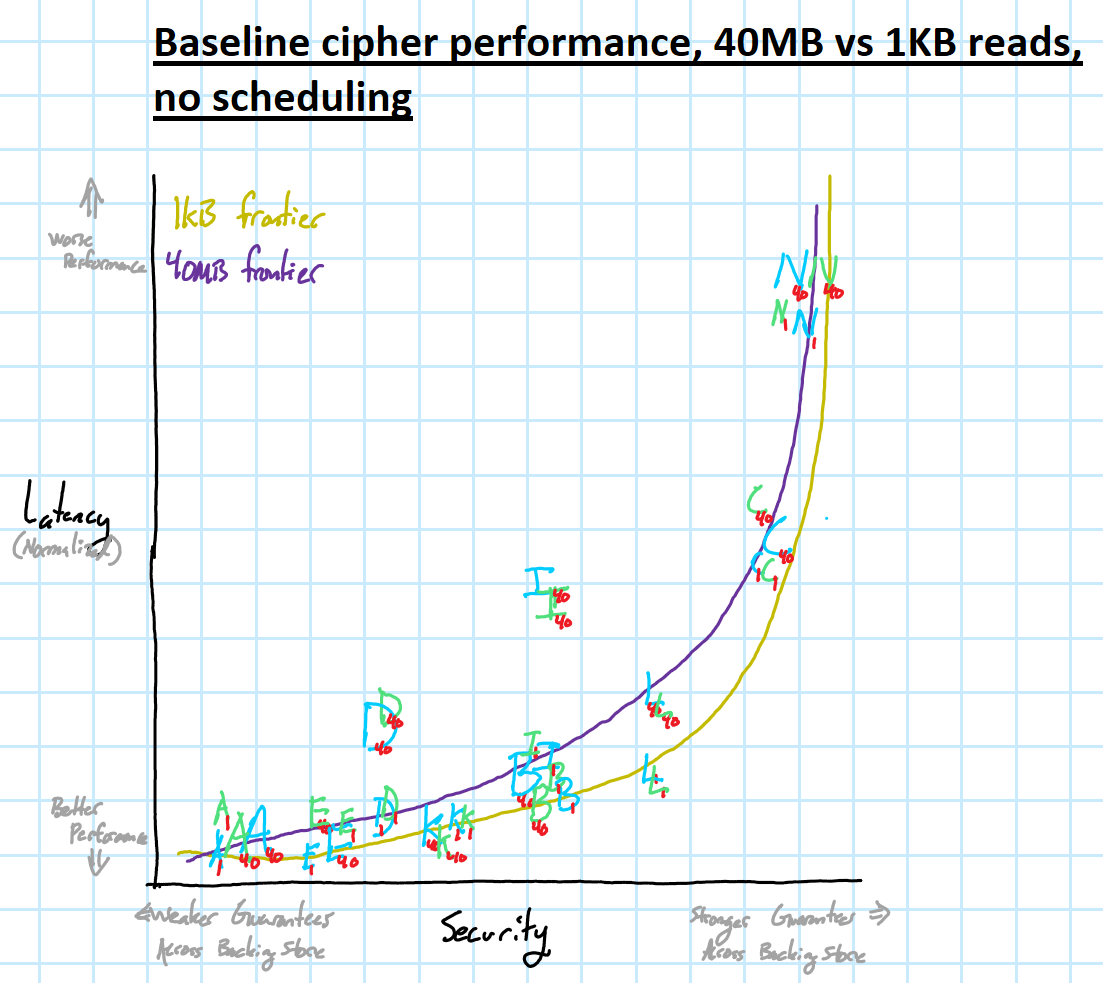
\includegraphics[width=\linewidth]{drawn/2.png}
   \caption{\TODO{Caption goes here}\TODO{Necessary chart? Or should we delete it and simply explain the curves are congruent with the original?}}\label{fig:40mb-vs-1kb-read}
\end{figure}

\begin{figure}[ht]
 \centering
  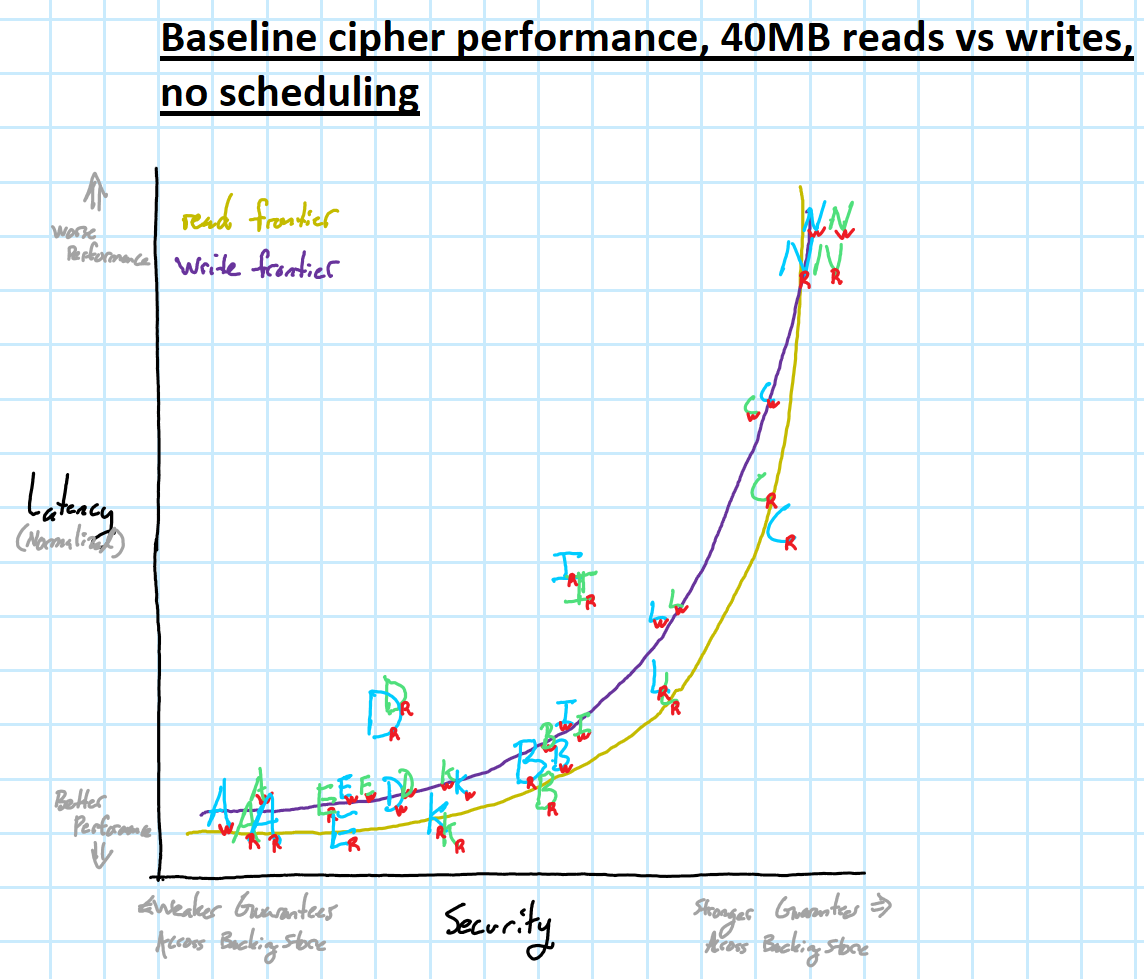
\includegraphics[width=\linewidth]{drawn/3.png}
   \caption{\TODO{Caption goes here}\TODO{Necessary chart? Or should we delete it and we simply explain the curves are congruent with the original?}}\label{fig:40mb-read-vs-write}
\end{figure}

\begin{figure}[ht]
 \centering
  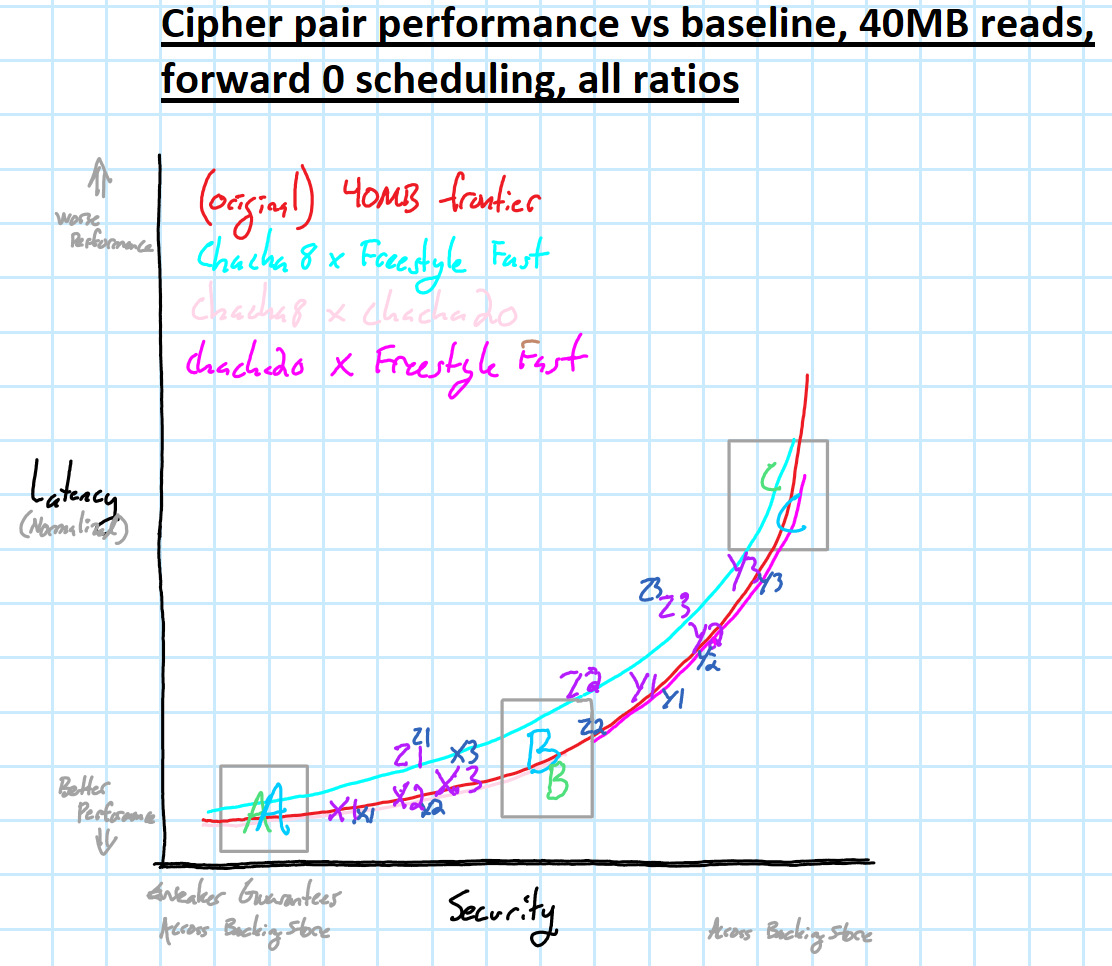
\includegraphics[width=\linewidth]{drawn/4.png}
   \caption{\TODO{Caption goes here}}\label{fig:navigating-the-space}
\end{figure}

\figref{navigating-the-space} shows the 40MB read performance of three ciphers:
ChaCha8, ChaCha20, and Freestyle in its "fast" configuration. This illustrates
the tradeoff space between latency/energy and security for these three static
discrete pareto optimal configurations achievable via prior work. On the other
hand, \figref{navigating-the-space} illustrates the flexibility of \SYSTEM{}
using the 0-forward switching strategy to reach dynamic configuration points
\emph{between} traditional static configuration in the tradeoff space that are
unachievable via prior work.

\TODO{Should there be a "ciphers" section somewhere that describes all the
various ciphers and cipher configurations? Would that best go in the design
section?}

\begin{figure}[ht]
 \centering
  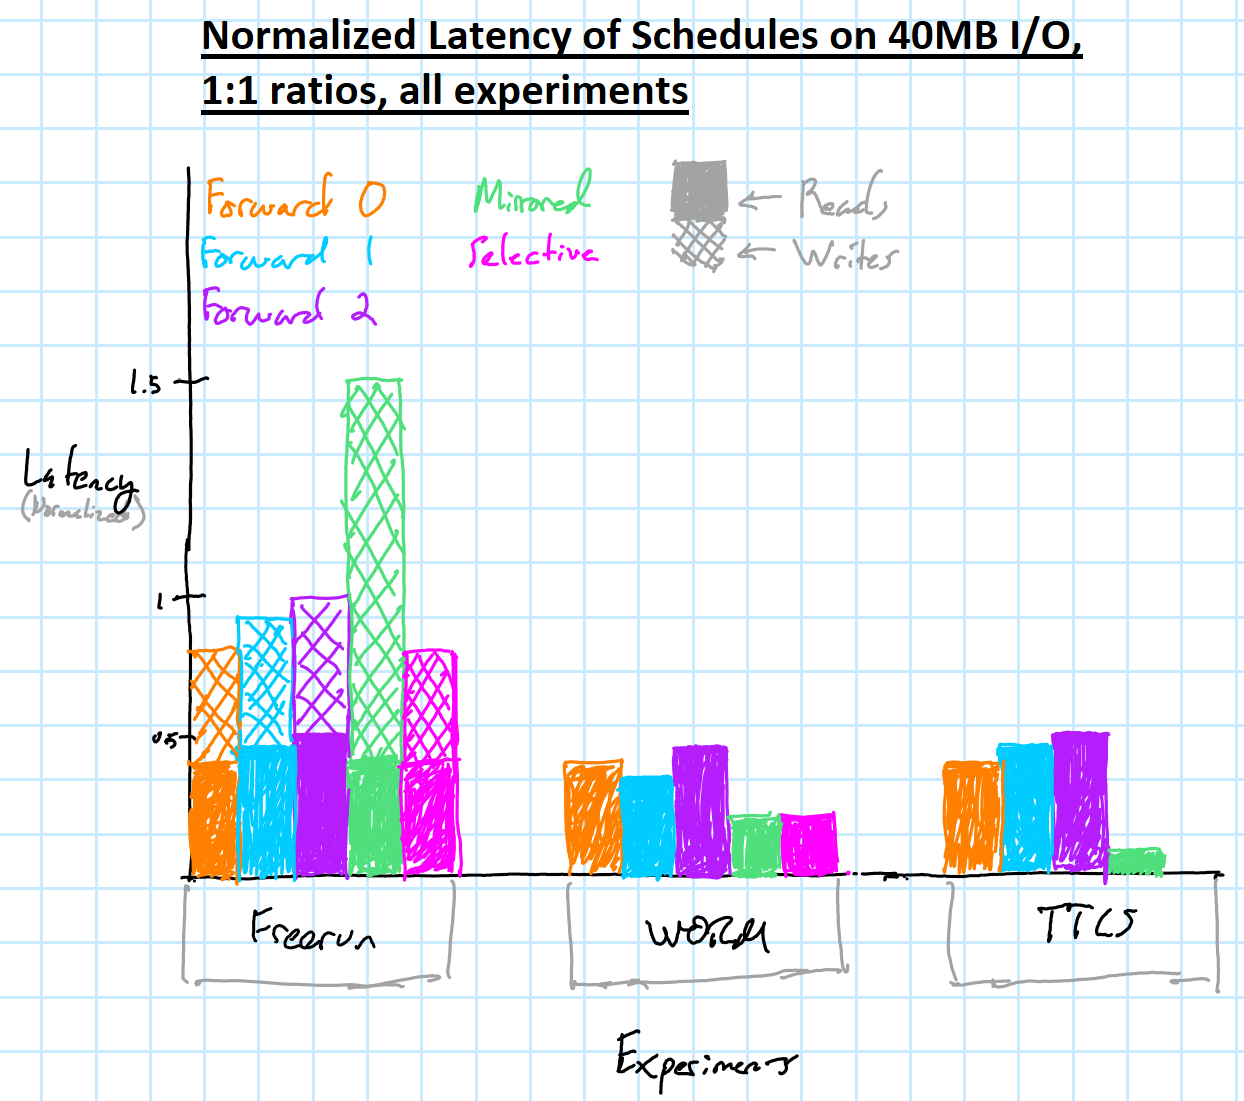
\includegraphics[width=\linewidth]{drawn/9.png}
   \caption{\TODO{Caption goes here}}\label{fig:strategy-vs-strategy}
\end{figure}

\TODO{Evaluate switching strategies against themselves. Different workloads,
different size, etc. Show that overhead is low. Show that performance is
maintained.}

\TODO{Paper up until this point makes assertions about static, offline, not
flexible. Evaluation shows flexibility.}

\TODO{Show the graph that demonstrates that we have a method to navigate this
space.}

\TODO{What assertions were made? Show results that demonstrate this.}

\TODO{This stuff works. Next section, show usefulness in practical
circumstances.}

\TODO{A point somewhere about when to use different strategies. List of concerns
that determine when to switch to what and why.}
